\documentclass[12pt]{report}

\usepackage{setspace}
%\setstretch{2.5} % for custom spacing
\setlength{\parindent}{4em}

\usepackage{fancyvrb}
\usepackage{graphicx}
\usepackage{geometry}

\geometry{letterpaper, portrait, margin=1in}

%%%Title Page%%%
\title{
  Lab 05
\bigbreak Digital Temperature Measurement and Display System Using the AD590 and the MC68HC11's A/D Converter
}

\author{
{\normalsize
\begin{tabular}{l r}
& \textbf{Zachary Davis}\\
\textbf{Category} & zachdav@uga.edu\\
\hline
Lab Part 1 & Software Development\\
Lab Part 2 & Hardware Development\\
Lab Part 3 & Calibrating The Measurement\\
\end{tabular}
}
}

\date{\bigskip
\today}
%%%%%%%%%%%%


\begin{document}
\maketitle
\section*{Introduction}
	\paragraph*{}
		The project presents a design that uses the temperature measurement of the AD590, read in and manipulated data by the HC11 itself and the A/D converter, as well as display the 
		output to the terminal for the end user.  More specifically, using an analog signal interface circuit to condition the current output by the AD590 and the A/D converter of the HC11, 	
		this project is able to display the digital temperature of the sensor and represent it with a number of LEDs.
	\paragraph*{}
		This is the first project that combines hardware design and software on the 68HC11.  This project has combined all the elements of previous projects from the binary to binary coded 
		decimal subroutine to how to print out formatted numbers.  With the previous knowledge I was able to focus on the three goals of this project.  Converting an analog signal to a 
		digital one, manipulate and calibrate that signal, and display the output to the user in the terminal and with the LEDs.
\section*{Lab Procedure}
	\paragraph*{}
		This project began with the design of a very basic flowchart far more simplistic than the on in appendix C.  The basic idea was to call on the HC11's A/D converter and redefine the 
		range from the standard 8 bit 0 - 255 range to one that represent 0 - 102.00 degrees celsius.  This was then returned back to the user through the terminal.  The temperature 
		measurements were sampled and echoed to the terminal every time the user inputs a character into the terminal.  This did not include the calibration of the temperature sensor or 
		the LED lights representing temperature.  
	\paragraph*{}
		From her came the development of the LED subroutine.  The idea was similar to what I did when converting the digital input to degrees celsius.  There are 9 states of the LEDs, 0 - 8
		LEDs illuminated.  By dividing the converted temperature by 9 it can then be compared to 9 even thresholds.  If the divided temperature is larger then one of these thresholds then 
		that determines how many LEDs to illuminate.  Essentially what I am doing is converting a range of 0 - 10200 degrees celsius to 0 - 9 LEDs.
	\paragraph*{}
		Once the basis for the software was completed the next step was to build the interface circuit that would comvert the output current by the AD590 to a voltage that range from 0 - 
		5 volts.  That range would align with the range of the A/D converter.  At this point that software and hardware were behaving as intended and although the temperature 
		measurements are very precise they were not accurate.  To do this measurements were taken from 30 - 80 degrees celsius and were used to generate an equation that would 
		calibrate the input readings.  After the calibration the same range of data points were measured again and were far more accurate and the difference could be accredited to 
		experimental error.  However, if I were doing this again i would use the second graph of data point to even further calibrate and tune the output temperature readings.
	\paragraph*{}
		The error in the A/D conversion is caused by many issues.  Initially the current that is output by the sensor and the actual temperature do not align and calibration is necessary to 
		correct this issue.  If not corrected to the higher the temperature the larger the propagation of error in the sensor which is why a slope intercept equation is required rather than 
		just an offset.  Once calibrated there are other sources of error in the A/D conversion.  Like with all measurements there is a portion of systematic error, which includes the many 
		environmental factors that skew the results like the tolerance of the temperature sensor as well as random error, or statistical fluctuations in measured data points.  These same to 
		factors effect the A/D converter itself.  Combined, even after calibration, these factors will have caused the error seen in appendix E.
	\paragraph*{}
		This lab report has easily been the most benefitial to any of those I have previously done.  Its foundation was build on everything we had previously learned and added to it the 
		use of the analog to digital conversion.  This lab continued to use the binary to binary coded decimal, BUFFALO I/O utility subroutines, and formatted outputs to the terminal I had 
		developed earlier, while causing me to apply it in a new way.  My knowledge of the A/D converter on the 68HC11 or any analog to digital converter was surface level.  I understood 
		that it was continuous versus digital and important topic covered in class, but I lacked a thurough understands of how it actually worked.  This lab gave that to me.  I now have a full
		and complete understanding of all the step required in an analog to digital conversion both with the HC11 and on a broader scale.  This includes things like the A/D control register 
		initiating the process, the delay required to complete the sampling, and interface circuit to condition the signal.  This lab was also able to give me a better understanding for the 
		AD590 temperature sensor and how to calibrate and handle error when converting from analog to digital.  Lastly, there were a lot of hardware reliability issues throughout this lab 
		and although very frustrating looking back on it, it did expand many skills with building circuits.  Not only was I required to complete the circuit, but had to carry out many methods of
		 error checking to find dead hardware or my error.
\section*{Conclusion}
	\paragraph*{}
		The purpose of this report was to discuss the temperature measurement and display laboratory.  Both the contruction of the hardware and the development of the software goals 
		were completed and the curcuit I built in tandom with the HC11 is able to measure the temperature both accurately and precisely and indicate that temperature numberically through
		 the terminal and visually through the EVB boards LEDs.  This lab was the first lab that combined my growing knowledge with the HC11 and assembly language with external 
		 hardware and introduced me to the analog to digital converter.  The lab taught me how to read in analog signals from a sensor and view the measurements on a host computer.  
		 On top of expanding my knowledge of A/D conversion in a very general way it also showed me the wide range of applications of circuits and software similar to those developed in 
		 this lab.

\section*{References}
	\paragraph*{}
		N/A

\section*{Appendix A: Hardware Schematic}
	\begin{center}
		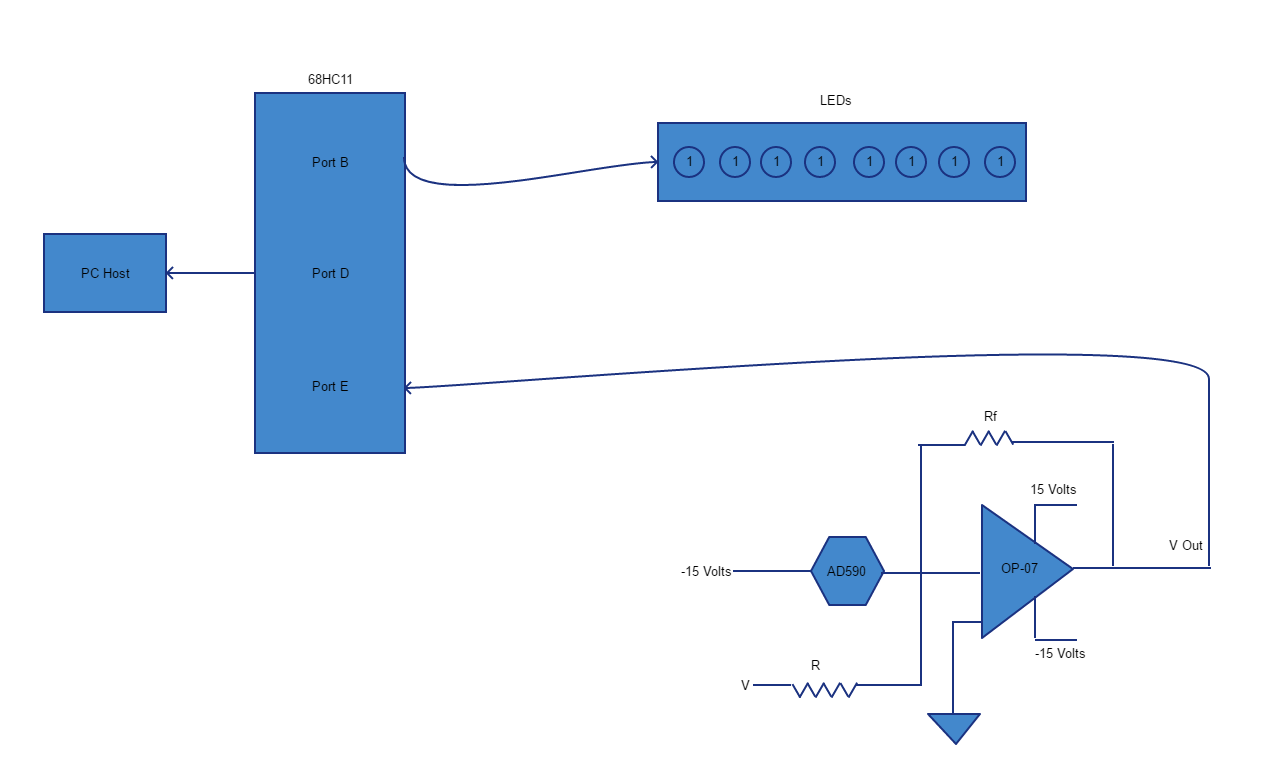
\includegraphics[scale=.50]{h.PNG}
	\end{center}

\section*{Appendix B: Pseudo Code For The Software Developed}
	\begin{Verbatim}[frame=single, fontsize=\small]
Define the ASCII output BUFFALO utility subroutines and INCHAR subroutine.
Define the address of PortB and Address of the result of the A/D converter.
Define the control register to read in single channel, one time, from the PE3 Pin
Define a variable to contain the temperature read in by the sensor.
		
Begin the MAIN portion of the code:
Prompt the user asking to take a signal from the A/D converter.
Await for the character input from the user.
Store the control settings at the A/D control register address.
Loop just over 128 clock cycles to wait for the A/D converter to complete.
Convert the input digital value to a calibrated temperature.
Convert the temperature value to binary coded decimal.
Echo the value of the temperature back to the terminal of the host PC.
Illuminate a relative portion of LEDs to represent the temperature read in.
Loop back to the beginning of the MAIN portion of code.
		
Convertion:
Scale the 0-255 digital range to 0-10200 degrees celsius by multiplying by 40.
Generate a Y=mX+B equation to calibrate the rescaled input.
Store this in temperature.
		
BinBCD:
Convert the rescaled and calibrated temperature to binary coded decimal.
Divide the temperature by a power of ten to isolate a digit.
Store the answer in the lower right nibble of an address.
Continue this until all five digits have been seperated and stored.
		
Print:
Load each of the address used to store the binary coded decimal digits.
Print out the right nibble of each of these address.
Print a decimal after three digits followed by the next to.  Convserves persicion
		
LED:
Divide the temperature by 9 (Number of LED groups).
Compare with predetermined thresholds until the number is greater than one.
Branch to the corresponding subroutine and light up the right number of LEDs.
	\end{Verbatim}
\section*{Appendix C: Program Flowchart}
	\begin{center}
		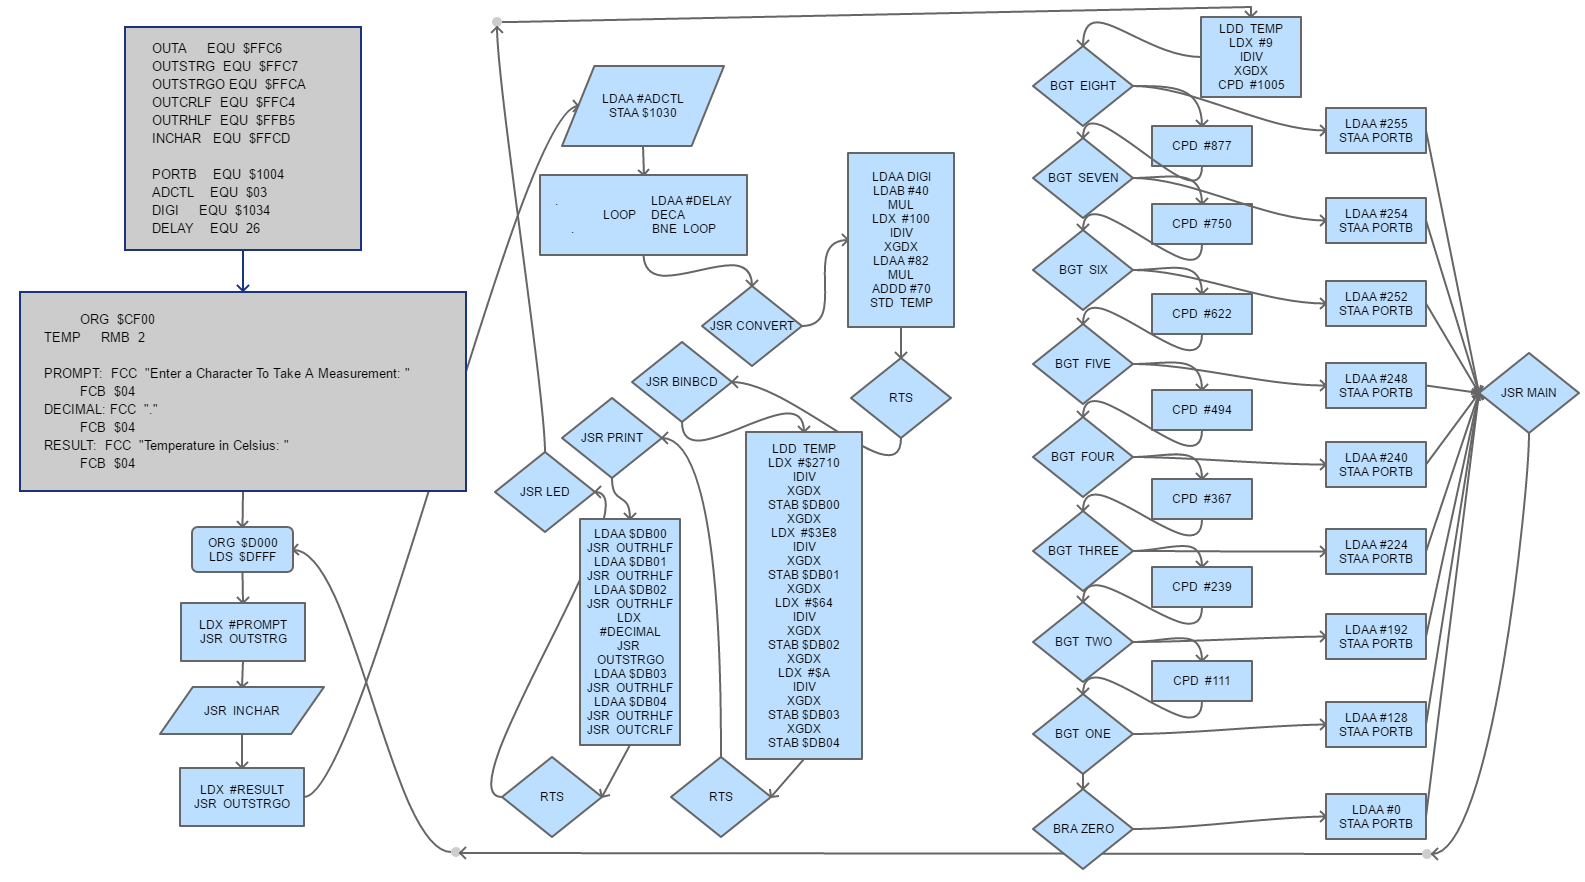
\includegraphics[scale=.40]{f.PNG}
	\end{center}

\section*{Appendix D: Program Listing}
	\begin{Verbatim}[frame=single, fontsize=\small]
;Defining 6 of the 17 BUFFALO utility subroutines.  Setting various labels to
;certain locations in the EPROM chip on the EVB board that correspond to each of
;the utility subroutines.
OUTSTRG  EQU  $FFC7  ;Outputs the ASCII string pointed to by the X Register.
OUTSTRGO EQU  $FFCA  ;The difference is excluding a leading return carriage.
OUTCRLF  EQU  $FFC4  ;Outputs only a return carriage.
OUTRHLF  EQU  $FFB5  ;Outputs the right nibble of A as an ASCII message.
INCHAR   EQU  $FFCD  ;Stores an input ASCII character into A and echos it back.

PORTB    EQU  $1004  ;Defining the location of PortB with a label
ADCTL    EQU  $03    ;Defining the analog to digital conditions.  This includes
                     ;not scanning, single channel, and pin PE3.
DIGI     EQU  $1034  ;When using PE3 the result is stored at this address.
DELAY    EQU  26     ;Defining the delay integer when waiting on the A/D.

         ORG  $CF00  ;Origin of memory.
TEMP     RMB  2      ;Reserving 2 bytes for the temperature. Max = 10,000.

;Defining various strings that will be used in the program.  This ranges from
;prompting the user to formatting the final output.
PROMPT:  FCC  "Enter a Character To Take A Measurement: "
         FCB  $04
DECIMAL: FCC  "."
         FCB  $04
RESULT:  FCC  "Temperature in Celsius: "
         FCB  $04

         ORG  $D000  ;Origin of the program.
         LDS  $DFFF  ;Defining and loading the stack.

;This is the main portion of the program that loops indefinitely and calls the
;other subroutines needed to complete the program.  This routine prompts the
;user for an input.  When recieved the conditions of the A/D control are defined
;and its result is stored.  This is then converted from mV to celsius and
;converted to binary coded decimal.  This is then echoed back to the terminal
;and the temperature relative to MAX is used to light up a portion of the LEDs.
MAIN:    LDX  #PROMPT   ;Loads IND X with the ASCII message defined above.
         JSR  OUTSTRG   ;Calls the BUFFALO utility to output to the terminal.
         JSR  INCHAR    ;Waits on a character input in the terminal.
         LDX  #RESULT   ;Loads IND X with the ASCII message defined above.
         JSR  OUTSTRGO  ;Calls the BUFFALO utility to output to the terminal.
         LDAA #ADCTL    ;Loads the A/D conditions defined above into ACC A.
         STAA $1030     ;Stores these conditions at the control register. This
                        ;initiates the convertion.

         ;Delay loop that waits just longer the 128 (132 exactly) clock cycles
         ;to wait on the A/D converter and sure that all the results have been
         ;stored.
         LDAA #DELAY    ;Loads ACC A with the value of DELAY.
LOOP     DECA           ;Decrements the value in ACC A by one.
         BNE  LOOP      ;If ACC A isn't 0 it branches back to the LOOP label.
         
         JSR  CONVERT   ;Calls the CONVERT subroutine.
         JSR  BINBCD    ;Calls the binary to binary coded decimal subroutine.
         JSR  PRINT     ;Calls the PRINT subroutine.
         JSR  LED       ;Calls the LED subroutine
         SWI            ;This interrupt and end should not be reached and are
         END            ;here only to follow standard format.  Just in case.
         
;This subroutine lights LEDs on the board based on the recieved temperature. The
;higher the temperature the more LEDs that are illuminated.  Since there are 8
;LEDs, I definined 9 groups. One for each LED and an all off state.  The
;temperature at this point has been formatted and is 0-100 degrees celcius*100.
;That means that TEMP can range from 0-10,000. It is then divided by 9. The
;result is then compared to each of the 9 even distributed thresholds and if it
;is greather then the threshold the program branches to the appropriate group.
LED:     LDD  TEMP    ;Load ACC D with the value at TEMP.
         LDX  #9      ;Loads IND X with the number 9.
         IDIV         ;Divids the value in ACC D by the value in IND X.
         XGDX         ;Swaps the value of ACC D and IND X.
         CPD  #1005   ;Compare ACC D to a threshold.
         BGT  EIGHT   ;If greater then zero 8 LEDs are illuminated.
         CPD  #877    ;Compare ACC D to a threshold.
         BGT  SEVEN   ;If greater then zero 7 LEDs are illuminated.
         CPD  #750    ;Compare ACC D to a threshold.
         BGT  SIX     ;If greater then zero 6 LEDs are illuminated.
         CPD  #622    ;Compare ACC D to a threshold.
         BGT  FIVE    ;If greater then zero 5 LEDs are illuminated.
         CPD  #494    ;Compare ACC D to a threshold.
         BGT  FOUR    ;If greater then zero 4 LEDs are illuminated.
         CPD  #367    ;Compare ACC D to a threshold.
         BGT  THREE   ;If greater then zero 3 LEDs are illuminated.
         CPD  #239    ;Compare ACC D to a threshold.
         BGT  TWO     ;If greater then zero 2 LEDs are illuminated.
         CPD  #111    ;Compare ACC D to a threshold.
         BGT  ONE     ;If greater then zero 1 LEDs are illuminated.
         BRA  ZERO    ;0 LEDs are illuminated.
         SWI          ;This should never be reached and is here just in case.
                      ;The branched subroutines return to the MAIN.

;These are the 9 LED groups, whose label correlates to the number of LEDs that
;should be illuminated from left to right.  Each of the 8 bits represents an LED
;(1 = on and 0 = off). This value is then stored at the address of Port B. This
;is the last task the program should complete and thus jumps back to MAIN to
;start the whole process over again.
EIGHT:   LDAA #255    ;Load ACC A with %11111111.
         STAA PORTB   ;Stores this value at PortB.
         JMP  MAIN    ;Returns to the MAIN label as this was the final task.
SEVEN:   LDAA #254    ;Load ACC A with %11111110.
         STAA PORTB   ;Stores this value at PortB.
         JMP  MAIN    ;Returns to the MAIN label as this was the final task.
SIX:     LDAA #252    ;Load ACC A with %11111100.
         STAA PORTB   ;Stores this value at PortB.
         JMP  MAIN    ;Returns to the MAIN label as this was the final task.
FIVE:    LDAA #248    ;Load ACC A with %11111000.
         STAA PORTB   ;Stores this value at PortB.
         JMP  MAIN    ;Returns to the MAIN label as this was the final task.
FOUR:    LDAA #240    ;Load ACC A with %11110000.
         STAA PORTB   ;Stores this value at PortB.
         JMP  MAIN    ;Returns to the MAIN label as this was the final task.
THREE:   LDAA #224    ;Load ACC A with %11100000.
         STAA PORTB   ;Stores this value at PortB.
         JMP  MAIN    ;Returns to the MAIN label as this was the final task.
TWO:     LDAA #192    ;Load ACC A with %11000000.
         STAA PORTB   ;Stores this value at PortB.
         JMP  MAIN    ;Returns to the MAIN label as this was the final task.
ONE:     LDAA #128    ;Load ACC A with %10000000.
         STAA PORTB   ;Stores this value at PortB.
         JMP  MAIN    ;Returns to the MAIN label as this was the final task.
ZERO:    LDAA #0      ;Load ACC A with %00000000.
         STAA PORTB   ;Stores this value at PortB.
         JMP  MAIN    ;Returns to the MAIN label as this was the final task.

;This subroutine outputs the digital temperature of the connected sensor. Binary
;to Binary Coded Decimal has already been completed when starting this
;subroutine and are stored from $DB00-$DB04. Each digit is stored in the right
;nibble and thus printed with OUTRHLF. The format is XXX.XX degrees celcius
;because when the signal was stored it was in mV and this was perserved to
;increase percision (Decimal place to the left 2x is the same as converting).
PRINT:   LDAA $DB00    ;Load ACC A with the value at $DB00.
         JSR  OUTRHLF  ;The right nibble is output to the terminal.
         LDAA $DB01    ;Load ACC A with the value at $DB01.
         JSR  OUTRHLF  ;The right nibble is output to the terminal.
         LDAA $DB02    ;Load ACC A with the value at $DB02.
         JSR  OUTRHLF  ;The right nibble is output to the terminal.
         LDX  #DECIMAL ;Loads an ASCII "." into IND X.
         JSR  OUTSTRGO ;The BUFFALO utility prints the ASCII string in IND X.
         LDAA $DB03    ;Load ACC A with the value at $DB03.
         JSR  OUTRHLF  ;The right nibble is output to the terminal.
         LDAA $DB04    ;Load ACC A with the value at $DB04.
         JSR  OUTRHLF  ;The right nibble is output to the terminal.
         JSR  OUTCRLF  ;A return carriage is output to the terminal for format.
         RTS           ;Return to the MAIN from this subroutine.

;This subroutine formats a value in Binary Coded Decimal.  Specifically it
;converts the temperature read in from the sensor to Binary Coded Decimal. This
;format can then be printed by the PRINT subroutine to show the result in the
;terminal to the user.
BINBCD:  LDD  TEMP    ;Loads ACC D with the value at TEMP.
         LDX  #$2710  ;Loads IND X with the value 10,000.
         IDIV         ;Divides the value in ACC D with the value in IND X.
         XGDX         ;Swaps ACC D with IND X.
         STAB $DB00   ;Stores the leading digit at $DB00.
         XGDX         ;Swaps ACC D with IND X.
         LDX  #$3E8   ;Loads IND X with the value 1,000.
         IDIV         ;Divides the value in ACC D with the value in IND X.
         XGDX         ;Swaps ACC D with IND X.
         STAB $DB01   ;Stores the leading digit at $DB01.
         XGDX         ;Swaps ACC D with IND X.
         LDX  #$64    ;Loads IND X with the value 100.
         IDIV         ;Divides the value in ACC D with the value in IND X.
         XGDX         ;Swaps ACC D with IND X.
         STAB $DB02   ;Stores the leading digit at $DB02.
         XGDX         ;Swaps ACC D with IND X.
         LDX  #$A     ;Loads IND X with the value 10.
         IDIV         ;Divides the value in ACC D with the value in IND X.
         XGDX         ;Swaps ACC D with IND X.
         STAB $DB03   ;Stores the leading digit at $DB03.
         XGDX         ;Swaps ACC D with IND X.
         STAB $DB04   ;Stores the leading digit at $DB04.
         RTS          ;Return to the MAIN from this subroutine.

;This subroutine converts the input converted digital voltage to degrees celsius
;as well as implement an equation to calibrate the sensor (Y=0.82X+0.70). By
;multiplying DIGI (0-255) by 40 and dividing by 100 TEMP is now 0-102 degrees
;celsius.  Finally multiplying it by 82 (slope) and adding 70 (intercept) to
;store the converted and calibrated value at TEMP.  Mulitplying by 40 converts
;the 0-255 input to mC.  It is then essenially multiplied by 82/100 or 0.82 and
;adding 70 or 0.70.  This is done because numbers < 1 but > 0 cannot be
;represented.  Lastly these muliplications are split up by a division in order
;to keep the result from going out of range of ACC D and IND X (65,535).
CONVERT: LDAA DIGI   ;Loads ACC A with the digital value read in from the A/D.
         LDAB #40    ;Loads ACC B with 40.
         MUL         ;Multiplies ACC A and ACC B.
         LDX  #100   ;Loads IND X with the value of 100.
         IDIV        ;Divides the value of ACC D with the value of IND X.
         XGDX        ;Swaps ACC D with IND X.
         LDAA #82    ;Loads ACC A with the value 82 (ACC B contain rNibble D).
         MUL         ;Multiplies ACC A and ACC B.
         ADDD #70    ;Adds the equivilent of 0.70 to ACC D.
         STD  TEMP   ;Stores this final value in variable TEMP.
         RTS         ;Return to the MAIN from this subroutine.
	\end{Verbatim}
	
\section*{Appendix E: Temperature Measurements}
	\begin{center}
		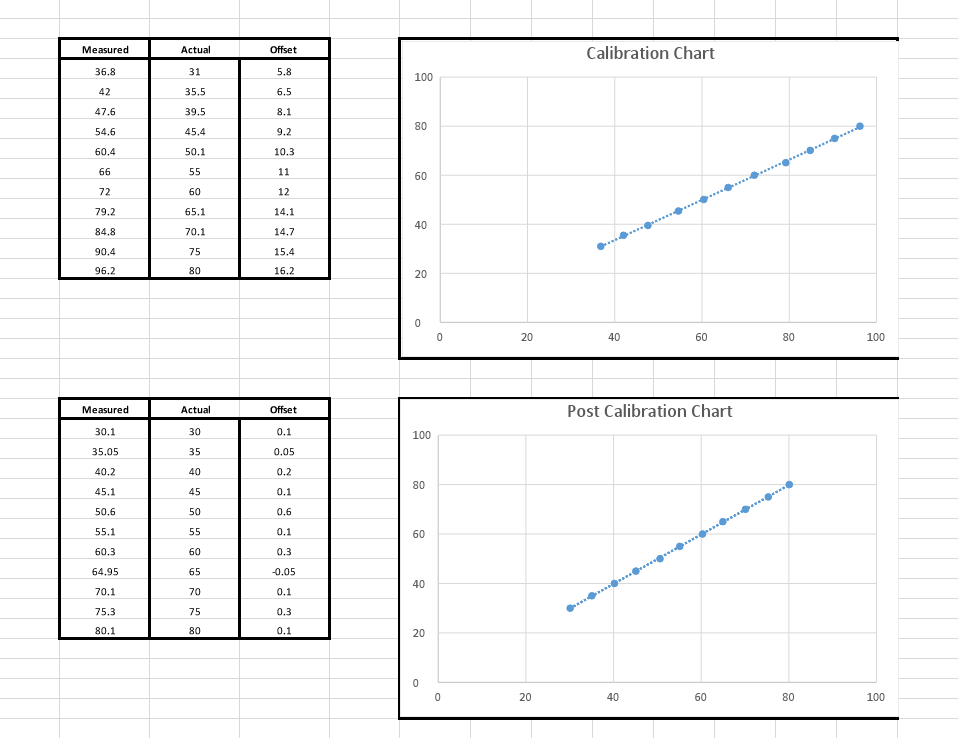
\includegraphics[scale=.60]{c.PNG}
		Calibration Equartion $Y = 0.8205x + 0.7035$
	\end{center}
\end{document}